\textcolor{blue}{Problem 1}

9.1 Channel with two independent looks at $Y$. Let $Y_1$ and $Y_2$ be conditionally independent and conditionally identically distributed given $X$.

(a) Show that $I\left(X ; Y_1, Y_2\right)=2 I\left(X ; Y_1\right)-I\left(Y_1 ; Y_2\right)$.

(b) Conclude that the capacity of the channel \\
\begin{figure}[htbp]
    \centering
	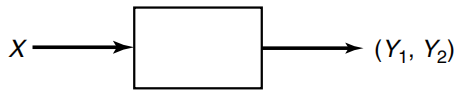
\includegraphics[width=0.4\textwidth]{../figure/9_1_9_2.png}
\end{figure}

is less than twice the capacity of the channel

\begin{figure}[htbp]
    \centering
	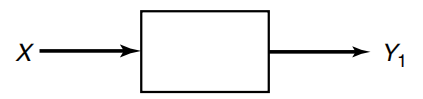
\includegraphics[width=0.37\textwidth]{../figure/9_1.png}
\end{figure}

\textcolor{blue}{Solution}

(a) \begin{align*}
I\left(X ; Y_1, Y_2\right) &= h\left(Y_1, Y_2\right) - h\left(Y_1, Y_2 | X\right) \\
&= h\left(Y_1, Y_2\right) - h\left(Y_1 | X\right) - h\left(Y_2 | X\right) \qquad\qquad\qquad\qquad\quad \left(\text{Since } Y_1\perp Y_2 | X \right) \\
&= h(Y_1, Y_2) + I(X,Y_1) - h(Y_1) + I(X;Y_2) - h(Y_2) \qquad \left(\text{Since } I(X;Y_i)=h(Y_i)-h(Y_i|X) \right) \\
&= I(X;Y_1) + I(X;Y_2) - \left(h(Y_1) + h(Y_2) - h(Y_1, Y_2)\right) \\
&= 2I(X;Y_1) - I(Y_1;Y_2) \qquad\qquad\qquad\qquad\qquad\qquad\quad\ \ \left(\text{Since } Y_1, Y_2 \text{ are identical distributed when given } X \right)
\end{align*}

(b) Suppose the channel capacity of the first channel is $C_1$ and the second channel is $C_2$. Then, we have
\begin{align*}
C_1 &= \max_{p(x)}\ I(X;Y_1,Y_2) \\
&= \max_{p(x)}\ 2I(X;Y_1) - I(Y_1;Y_2) \\
&\leq \max_{p(x)}\ 2I(X;Y_1) \qquad \left(\text{Since } I\left(Y_1,Y_2\right)\geq 0 \right) \\
&= 2\max_{p(x)}\ I(X;Y_1) \\
&= 2C_2
\end{align*}
If and only if $I(Y_1;Y_2)=0$, i.e. $Y_1\perp Y_2$, the equality holds.

So above all, we have proved that the capacity of the channel is less than twice the capacity of the channel.

\newpage